\documentclass[tikz,convert={outext=.svg,command=\unexpanded{pdf2svg \infile\space\outfile}},multi=false]{standalone}
\usepackage[utf8]{inputenc}

\usetikzlibrary{automata}% tikz package already loaded by 'tikz' option

\begin{document}

\begin{tikzpicture}
\node (avant) at (0, 5) {
\begin{tikzpicture}
\tikzstyle{state} = [draw, circle, fill=white];
\tikzstyle{init} = [initial, initial text={}];
\tikzstyle{final1} = [draw=blue, double];
\tikzstyle{final2} = [draw=red, double];
\node[state, init] (q0) {$q_0$};
\node[state, final1] (q1) at (-2, -2) {$q_1$};
\node[state, final2] (q2) at (2, -2) {$q_2$};
\draw[->] (q0) edge[loop above] node {$\top$} (q0);
\draw[->] (q0) edge[bend right=20] node[left] {$cr_1$} (q1);
\draw[->] (q0) edge[bend left=20] node[right] {$cr_2$} (q2);
\draw[->] (q1) edge[bend right=20] node[right] {$\top$} (q0);
\draw[->] (q2) edge[bend left=20] node[left] {$\top$} (q0);
\end{tikzpicture}};



\node (apres) at (0, -3) {
	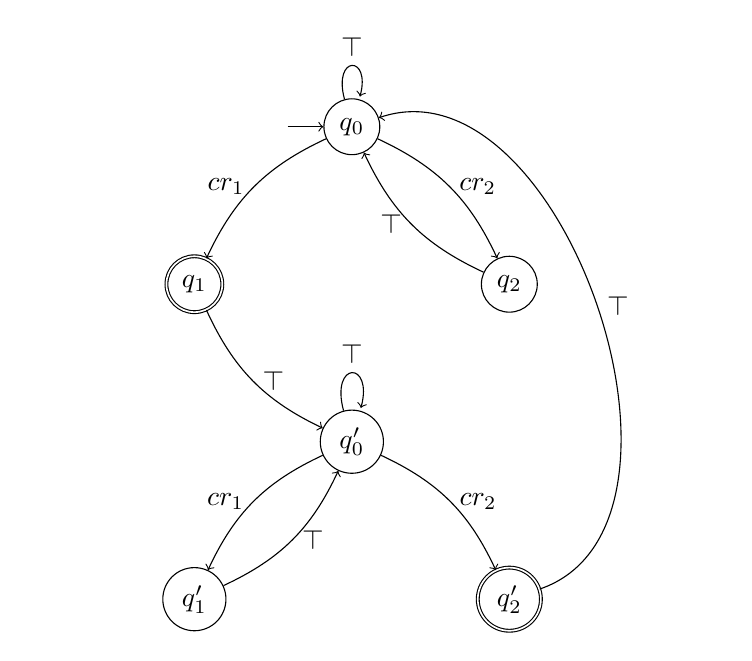
\begin{tikzpicture}
	\node at (-4,0) {};
\tikzstyle{state} = [draw, circle, fill=white];
\tikzstyle{init} = [initial, initial text={}];
\tikzstyle{final} = [double];
\tikzstyle{final2} = [double];
\node[state, init] (q0) {$q_0$};
\node[state, final] (q1) at (-2, -2) {$q_1$};
\node[state] (q2) at (2, -2) {$q_2$};
\draw[->] (q0) edge[loop above] node {$\top$} (q0);
\draw[->] (q0) edge[bend right=20] node[left] {$cr_1$} (q1);
\draw[->] (q0) edge[bend left=20] node[right] {$cr_2$} (q2);
%
\draw[->] (q2) edge[bend left=20] node[left] {$\top$} (q0);

\node[state] (2q0) at (0, -4) {$q_0'$};
\node[state] (2q1) at (-2, -6) {$q_1'$};


\draw[->] (q1) edge[bend right=20] node[right] {$\top$} (2q0);


\node[state,final] (2q2) at (2, -6) {$q_2'$};
\draw[->] (2q0) edge[loop above] node {$\top$} (2q0);
\draw[->] (2q0) edge[bend right=20] node[left] {$cr_1$} (2q1);
\draw[->] (2q0) edge[bend left=20] node[right] {$cr_2$} (2q2);
\draw[->] (2q1) edge[bend right=20] node[right] {$\top$} (2q0);
\draw[->] (2q2) edge[bend right=90] node[right] {$\top$} (q0);
\end{tikzpicture}};

\draw[line width=2mm,-latex] (avant) edge (apres);

\end{tikzpicture}
\end{document}